\chapter{Design Patterns}

\section{Overview}

A \emph{design pattern}\index{design pattern}
is a proven solution to a recurring
problem in software design and development.
A typical pattern is not reusable code, as a library function would be,
but consists of problems, motivations, and design decisions
related to the elements of a software artifact.
Many functional logic design patterns are centered on the characteristic
features of the paradigm, non-determinism and logic variables.

Patterns originated for object-oriented programming languages
and became an important discipline in computer
science after \cite{GammaEtAl94}.
Design patterns for functional logic programming
were introduced and further developed in
\cite{AntoyHanus02FLOPS,AntoyHanus11WFLP}.
We present a pattern using \emph{tags}\index{pattern!tag},
typically a one-line description of some key element
of a problem or its solution.
In this tutorial, we use only four simple tags:
\emph{name}\index{pattern!name},
\emph{intent}\index{pattern!intent},
\emph{solution}\index{pattern!solution}, and
\emph{structure}\index{pattern!structure}
with self-explaining meaning.

\subsection{Deep selection}\label{sec-Deep-selection}

\begin{center}
\begin{tabular}{@{} | *{2}{@{\hspace{3pt}} l @{\hspace{3pt}} |} @{}}
\hline
Name & \emph{Deep selection} \\
\hline 
Intent & pattern matching at arbitrary depth in recursive types \\
\hline
Applicability & select an element with given properties in a structure \\
\hline
Structure & combine a type generator with a functional pattern \\
\hline
\end{tabular}
\end{center}

\noindent
Recursively defined
types, such as lists and trees, have components at arbitrary
depths that cannot be selected by pattern matching because pattern
matching selects components only at predetermined positions.  
For recursively defined types, the
selection of some element with a given property in a
data structure typically requires code for the traversal of the
structure which is intertwined with the code for using the element.  The
combination of functional patterns with type generators
allows us to select elements arbitrarily nested in a
structure in a pattern matching-like fashion without
explicit traversal of the structure and mingling of
different functionalities of a problem.

We show the application of this pattern in one example.
Consider a simple type for representing arithmetic
expressions:
%
\begin{prog}
data Exp = Lit Int
         | Var [Char]
         | Add Exp Exp
         | Mul Exp Exp
\end{prog}
%
For example, the expression $x+1$ is encoded as 
$e = \code{Add (Var "x") (Lit 1)}$.
Suppose that we want to match an expression with 
some property, e.g., the expression is a variable,
regardless of whether it occurs.
First, we define a function, \emph{withSub},
that takes an expression $t$
and non-deterministically generates 
some expression with $t$ as subexpression.
%
\begin{prog}
withSub exp = exp
            ? op (withSub exp) unknown
            ? op unknown (withSub exp)
   where op = Add ? Mul  
\end{prog}
%
For example, if $t = \code{Var "x"}$, then
\code{withSub $t$} evaluates, among other possibilities,
to an expression matching the expression $e$ discussed earlier.
Thus, using functional patterns, Sect.~\ref{Functional Patterns},
we can pattern match a subexpression $t$ anywhere in an expression $e$.

To see this in action, consider the function \emph{varOf} defined below.
This function takes an expression $e$ and returns  the identifier
of a variable occurring anywhere in $e$.  With ordinary pattern matching,
only a variable at a fixed position, e.g., the root or the left
argument of an expression, can be matched.  With \emph{withSub} we
match any variable anywhere:
%
\begin{prog}
varOf :: Exp -> String
varOf (withSub (Var v)) = v  
\end{prog}
%
For example, the set of the identifiers of all the variables of
occurring in an expression $e$ is simply obtained with the set function
of \code{varOf}, i.e., \code{\funset{varOf} $e$}
\proghref{expr}{Program}.

\subsection{Constrained Constructor}\label{sec-constrained-constructor}

\begin{center}
\begin{tabular}{@{} | *{2}{@{\hspace{3pt}} l @{\hspace{3pt}} |} @{}}
\hline
Name & \emph{Constrained Constructor} \\
\hline 
Intent & prevent invoking a constructor that might create invalid data \\
\hline
Applicability & a type is too general for a problem \\
\hline
Structure & define a function that either invokes a constructor or fails \\
\hline
\end{tabular}
\end{center}
%
The signature of a functional logic program is partitioned into
\emph{defined operations} and \emph{data constructors}.
They differ in that operations manipulate data by means of rewrite rules,
whereas constructors create data and have no associated rewrite rules.
Therefore, a constructor symbol cannot perform any checks on the
arguments to which it is applied.  If a constructor is invoked
with arguments of the correct types, but inappropriate values,
conceptually invalid data is created.
We use an example to clarify this point.

The \emph{Missionaries and Cannibals} puzzle is stated as follows.
Three missionaries and three cannibals want to cross a river
with a boat that holds up to two people.
Furthermore, the missionaries, if any, on either bank of the river
cannot be outnumbered by the cannibals
(otherwise, as the intuition hints, they would be eaten by the cannibals).

A state of this puzzle is represented by the number of
missionaries and cannibals and the presence of the boat on an
arbitrarily chosen bank of the river, by convention the \emph{initial} one:
%
\begin{prog}
data State = State Int Int Bool
\end{prog}
%
For example, with suitable conventions,
\code{(State 3 3 True)} represents the initial state.
The simplicity of this representation has the drawback
that invalid states, e.g., those with more than 6 people,
can be created as well.
Unless complex and possibly inefficient types for the state are
defined, it is not possible to avoid the creation of invalid states
using constructors alone.

The \emph{Constrained Constructor} pattern avoids
the creation of invalid states.
The programmer invokes the constructor indirectly
through the following function:
%
\begin{prog}
makeState m c b | valid \boolAnd safe = State m c b
   where valid = 0<=m \boolAnd m<=3 \boolAnd 0<=c \boolAnd c<=3
         safe  = m==3 || m==0 || m==c
\end{prog}
%
Function \code{makeState} invokes the constructor only
after checking that only states
that are consistent with the physical conditions of the
puzzle and are safe for the missionaries will be created.
For example, 
\code{(State 2 1 \panon)} is not safe since on one bank of the river
the cannibals outnumber the missionaries
and therefore should not be created.
In fact, the call \code{makeState\,2\,1\,\_} fails because
the rule's condition is not satisfied.
In a suitable non-deterministic program, this failure can be
simply and silently ignored.

Operation \code{makeState} eases the definition of an operation,
say \code{move}, to move people and boat across the river:
%
\begin{prog}
move (State m c True)
   = makeState (m-2) c False      \lineComment move 2 missionaries
   ? makeState (m-1) c False      \lineComment move 1 missionary
   ? makeState m (c-2) False      \lineComment move 2 cannibals
   ? ...
\end{prog}
%
since ``undesirable'' states are never produced
\proghref{missionaries}{Program}.

\subsection{Non-determinism introduction and elimination}
\label{Non-determinism introduction and elimination}

\begin{center}
\begin{tabular}{@{} | *{2}{@{\hspace{3pt}} l @{\hspace{3pt}} |} @{}}
\hline
Name & \emph{Non-determinism introduction and elimination} \\
\hline 
Intent & use different algorithms for the same problem \\
\hline
Applicability & some algorithm is too slow or it may be incorrect \\
\hline
Structure & either replace non-deterministic code with deterministic one or vice versa \\
\hline
\end{tabular}
\end{center}

Specifications are often non-deterministic because
in many cases non-determinism defines the desired results of
a computation more easily than by other means.
We have seen this practice in several previous examples.
Thus, it is not unusual for programmers to
initially code a non-deterministic prototype
even for deterministic problems because this approach
produces correct programs quickly.

In some cases, a non-deterministic program is not
efficient enough to solve a problem of interesting size.
Reducing the non-determinism of the program, e.g.,
by taking advantage of domain knowledge, 
may improve the efficiency of execution.
Below, is an example.
The ``\emph{blocks world}'' \cite{wiki:blocks-world}
consists of 3 possibly empty piles,
labeled $p$, $q$ and $r$,
of unique blocks labeled {\bf A}, {\bf B}, {\bf C}, etc.
``\emph{Start}'' and ``\emph{Final}'' below are two examples
of blocks worlds from \cite{Shute20blocks-world}.
%
\begin{center}
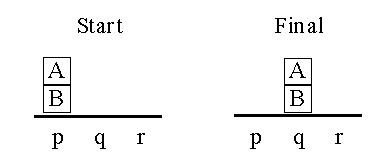
\includegraphics[scale=.5]{PICTURES/problem.jpg}
\end{center}
%
A blocks world ``\emph{problem}'' consists of two worlds,
like Start and Final above.
Its solution consists in the moves that produce the second world
from the first one.
A ``\emph{move}'' transfers the block on top of a pile
to the top of another pile. No other blocks are affected by the move.
Below is an example of a solution from Start to Final.
%
\begin{center}
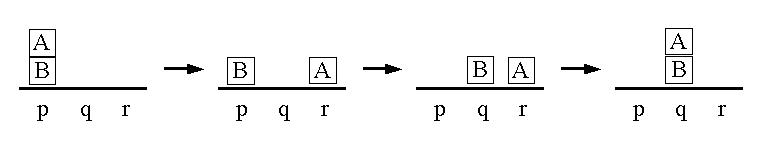
\includegraphics[scale=.5]{PICTURES/solution.jpg}
\end{center}
%
In our prototype,
blocks are encoded as an enumerated type.
A world is three stacks of blocks.
A solution is a sequence of worlds.
A problem is a pair of words.
%
\begin{prog}
data Block = A | B | C | D | E deriving Eq
type Stack = [Block]
type World = (Stack, Stack, Stack)
type Trace = [World]
data Problem = Problem World World
\medskip
simpleProblem, difficultProblem :: Problem
simpleProblem = Problem ([A,B],[],[]) ([],[A,B],[])
difficultProblem = Problem ([A,B,C,D,E],[],[]) ([],[C,B,A,D,E],[])
\end{prog}
%
We define two functions to solve a blocks world problem.
Function \code{move} moves the block at the top of a pile to
the top of another different pile.  Both the origin and the destination pile
of a move are non-deterministically selected.
Function \code{extend} takes a sequence of blocks world states,
that we call a \emph{trace}, that when reversed satisfies the
following invariant: (1) the first block is the start state,
(2) any other block is obtained from the previous one by a move,
and (3) no element, with the possible exception of the last one,
is repeated.

Function \code{extend} performs the following tests and corresponding
actions on the last element, $t$, of the trace (the first element actually,
since the trace is reversed):
(1) if $t$ is the final world, the trace is a solution,
(2) if $t$ is repeated in the trace, the computation is aborted,
otherwise (3) the trace is extended with a move from $t$:
%
\begin{prog}
move :: World -> World
move (x:xs, ys, zs) = (xs, x:ys, zs) ? (xs, ys, x:zs) -- p -> q/r
move (xs, y:ys, zs) = (y:xs, ys, zs) ? (xs, ys, y:zs) -- q -> p/r
move (xs, ys, z:zs) = (z:xs, ys, zs) ? (xs, z:ys, zs) -- r -> p/q
\medskip
extend :: Trace -> World -> Trace
extend trace@(t:ts) goal
  | t == goal    = reverse trace
  | t `elem` ts  = failed
  | otherwise    = extend (move t : trace) goal
\medskip
main :: Problem -> Trace
main = extend [s] f where Problem s f = simpleProblem
\end{prog}
%
The \pakcs{} interpreter produces 40 solutions of \code{simpleProblem}
in which the number of moves ranges from 3 to 10, in a fraction of a second.
However, it does not produce any solution of \code{difficultProblem} in
over an hour.  We are guessing that the reason is that the
non-determinism of \code{move} is too ``unfocused.''
\proghref{blocks}{Program}.

We reduce the non-determinism of the previous program using
two strategies.  We favor moves that put a block in its final place and
by we avoid moves that take a block away from its final place.
Function \code{moveToGoal} is quite similar to function \code{move}
of the previous program, but it moves a block only
if the block ends up into its final place.  If such a move is not available,
the move is computed by function \code{noMoveFromGoal}.
This function is again quite similar to \code{move},
but a block that is already in its final place is never moved.

Observe that \code{noMoveFromGoal} would fail if called on the
final state of a blocks world problem.  An invariant of this
and the previous program is that no move is attempted on any
final state.
%
\begin{prog}
moveToGoal :: World -> World -> World
moveToGoal (x:xs, ys, zs) (_, _++x:ys, _) = (xs, x:ys, zs) -- p -> q
moveToGoal (x:xs, ys, zs) (_, _, _++x:zs) = (xs, ys, x:zs) -- p -> r
moveToGoal (xs, y:ys, zs) (_++y:xs, _, _) = (y:xs, ys, zs) -- q -> p
moveToGoal (xs, y:ys, zs) (_, _, _++y:zs) = (xs, ys, y:zs) -- q -> r
moveToGoal (xs, ys, z:zs) (_++z:xs, _, _) = (z:xs, ys, zs) -- r -> q
moveToGoal (xs, ys, z:zs) (_, _++z:ys, _) = (xs, z:ys, zs) -- r -> p
moveToGoal'default w g = noMoveFromGoal w g
\medskip
noMoveFromGoal :: World -> World -> World
noMoveFromGoal (x:xs, ys, zs) (g, _, _)
  | not (isSuffixOf (x:xs) g) = (xs, x:ys, zs) ? (xs, ys, x:zs)
noMoveFromGoal (xs, y:ys, zs) (_, g, _)
  | not (isSuffixOf (y:ys) g) = (y:xs, ys, zs) ? (xs, ys, y:zs)
noMoveFromGoal (xs, ys, z:zs) (_, _, g)
  | not (isSuffixOf (z:zs) g) = (z:xs, ys, zs) ? (xs, z:ys, zs)
\medskip
extend :: Trace -> World -> Trace
extend trace@(t:ts) goal
  | t == goal    = reverse trace
  | t `elem` ts  = failed
  | otherwise    = extend (moveToGoal t goal : trace) goal
\medskip
main :: Trace
main = selectValue (set2 extend [s] f) 
     where Problem s f= difficultProblem
\end{prog}
%
The \pakcs{} interpreter produces 6 solutions of \code{simpleProblem}
in which the number of moves ranges from 3 to 7, in a fraction of a second.
It also produces a solution of \code{difficultProblem} in a few
seconds, but this solution is 170 moves long.  There exists a
solution of this problem which is only 12 moves long.
\proghref{betterblocks}{Program}.

The previous example and discussion shows that reducing the
non-determinism of a program may increase its efficiency.  Often, it
also increases its complexity. This patter comes in a dual form.
In some situations, e.g., if a program is producing unexpected
results, it may be useful to increase the program non-determinism.
This change will likely decrease the program efficiency,
but increase its simplicity.  With a simpler program it
may be easier to assess or verify whether a result of a computation
is expected.

